\documentclass{article}
\usepackage{amsmath} % need to be on top for eps files
\usepackage{caption}
\usepackage{subcaption}
\usepackage{graphicx}
\graphicspath{{latex/Images/}}
\usepackage{epstopdf}

%\usepackage[official]{eurosym}
%\usepackage{libertine}
\usepackage{textcomp}
\usepackage{eurosym}

\newcommand{\meuro}{\text{\euro}}
\makeatletter
% Definition taken from eurosym.sty, provides \EUR equivalent for math mode
\newcommand\MEUR[1]{\if@EURleft\text{\euro}\,\fi#1\if@EURleft\else\,\text{\euro}\fi}
\makeatother

%%%%%%%%%Custom
% Allow linking in document.
\usepackage{hyperref}

% Allow including autogenerated LaTex tables from Python.
\usepackage{booktabs}
\usepackage{longtable}
\usepackage{lipsum}

% Determine whether it is local compilation or overleaf compilation
\makeatletter
\begingroup\endlinechar=-1\relax
       \everyeof{\noexpand}%
       \edef\x{\endgroup\def\noexpand\homepath{%
         \@@input|"kpsewhich --var-value=HOME" }}\x
\makeatother
\def\overleafhome{/tmp}% change as appropriate

\ifx\homepath\overleafhome
    % Overleaf compilation.
    \newcommand\blockchaindev{76}
\newcommand\frontenddev{41}
\newcommand\humanresources{36}
\newcommand\totalcost{1359120}
 %\newpage
\else
    % Local compilation
    \newcommand\blockchaindev{76}
\newcommand\frontenddev{41}
\newcommand\humanresources{36}
\newcommand\totalcost{1359120}
 %\newpage
\fi

% Specify compilation name.
\def\filename{main}

% Specify what types of appendices are included in file.
\def\appendixtypes{no_code}
%\def\appendixtypes{project_code_only}
%\def\appendixtypes{export_code}
%\def\appendixtypes{project_and_export_code}



% Use H option in figure placement:
\usepackage{float}

% Use math letters
\usepackage{amsmath} % need to be on top for eps files
\usepackage{mathtools}

% Used for image geometry (already included)
%\usepackage{graphicx}

% Support auto referencing
\usepackage{cleveref}

\crefname{lstlisting}{listing}{listings}
\Crefname{lstlisting}{Listing}{Listings}

% Specify bibliography style:
\usepackage{url}

%%%%%%%%%End Custom


%%%%%%%%%%%%%%%%%%%%%%%%%%%%%%%%%%%%%%%%%%%%%%%%%% Create listings (Matlab)
% % Create a matlab listing
\usepackage{listings}
\usepackage{color} %red, green, blue, yellow, cyan, magenta, black, white
\definecolor{mygreen}{RGB}{28,172,0} % color values Red, Green, Blue
\definecolor{mylilas}{RGB}{170,55,241}

\usepackage[utf8]{inputenc}
\usepackage{geometry}
 \geometry{
 a4paper,
 total={175mm,265mm},
 left=15mm,
 top=15mm,
 }
\usepackage{amsmath}%To be able to use split in equation


%%%% Include eps files:
\usepackage{amsmath} % need to be on top for eps files
\usepackage{graphicx}
%set the relative location for eps files
\graphicspath{ {/Images/} }
\usepackage{listings}
\usepackage{cleveref} %cleverref needs to stand below amsmath package.
\usepackage{graphicx}
\usepackage{float}
%\usepackage{hyperref}
\usepackage{url} %To be able to use url in references
\usepackage{graphicx}
\usepackage{tabularx} % in the preamble
\usepackage{wrapfig}

% To get side by side pictures:{
\usepackage{caption}
\usepackage{subcaption}
\usepackage{graphicx}




%%%%%%%%%%%%%%%%%%%%%%%%%%%%%%%%%%%%%%%%%%%%%%%%%% Create listings (Python)
% set code color pattern (for python)
% Default fixed font does not support bold face
\DeclareFixedFont{\ttb}{T1}{txtt}{bx}{n}{12} % for bold
\DeclareFixedFont{\ttm}{T1}{txtt}{m}{n}{12}  % for normal

% Custom colors
\usepackage{color}
\definecolor{deepblue}{rgb}{0,0,0.5}
\definecolor{deepred}{rgb}{0.6,0,0}
\definecolor{deepgreen}{rgb}{0,0.5,0}

\usepackage{listings}

% Python style for highlighting
\newcommand\pythonstyle{\lstset{
language=Python,
breaklines=true, % wrap lines
postbreak=\mbox{\textcolor{red}{$\hookrightarrow$}\space}, % wrap lines
basicstyle=\ttm,
otherkeywords={self},             % Add keywords here
keywordstyle=\ttb\color{deepblue},
emph={MyClass,__init__},          % Custom highlighting
emphstyle=\ttb\color{deepred},    % Custom highlighting style
stringstyle=\color{deepgreen},
frame=tb,                         % Any extra options here
showstringspaces=false            %
}}

% Python environment
\lstnewenvironment{python}[1][]
{
\pythonstyle
\lstset{#1}
}
{}

% Python for external files
\newcommand\pythonexternal[2][]{{
\pythonstyle
\lstinputlisting[#1]{#2}}}

% Python for inline
\newcommand\pythoninline[1]{{\pythonstyle\lstinline!#1!}}


% Include path to images
\graphicspath{{Images/}{latex/project1/}}

% Include pdf files in report
\usepackage{pdfpages}


\usepackage{cleveref} %cleverref needs to stand below amsmath package.
\usepackage{appendix}
\crefname{appsec}{Appendix}{Appendices} % refer to appendix as appendix iso as section (use with text in
%\title{}
%\subtitle{}
\title{Roadmap: TruCol\\\large A decentralised collaboration protocol for test-driven development}
%\author{Authors:\\a-t-0}



%\def\parent_subpath{/latex/project}% change as appropriate (depending on what Overleaf does)
\usepackage{xstring}


%\def\project_one{/project1}% change as appropriate
%enable multirple columns
\usepackage{multicol}
\usepackage{multirow}

\usepackage{currfile}
\usepackage{currfile-abspath}

% use sidewaysfigure
\usepackage{rotating}

\date{\today}
\begin{document}
\crefname{lstlisting}{listing}{listings}
\Crefname{lstlisting}{Listing}{Listings}
%%%%%%%%%%Configure matlab listing%%%%%%%%%%%%%%%%%%
% Specify matlab listing style
\lstset{language=Matlab,%
    %basicstyle=\color{red},
    breaklines=true,%
    morekeywords={matlab2tikz},
    keywordstyle=\color{blue},%
    morekeywords=[2]{1}, keywordstyle=[2]{\color{black}},
    identifierstyle=\color{black},%
    stringstyle=\color{mylilas},
    commentstyle=\color{mygreen},%
    showstringspaces=false,%without this there will be a symbol in the places where there is a space
    numbers=left,%
    numberstyle={\tiny \color{black}},% size of the numbers
    numbersep=9pt, % this defines how far the numbers are from the text
    emph=[1]{for,end,break},emphstyle=[1]\color{red}, %some words to emphasise
    %emph=[2]{word1,word2}, emphstyle=[2]{style},
}


\maketitle
%\setcounter{chapter}{-1}

% Create abstract.
\ifx\homepath\overleafhome
    % Overleaf compilation.
    \section{Introduction}
This roadmap for the Seed Milestone Fund describes how TruCol got started, where we currently are, which milestones take us to a significant market share, and what capital is being raised now, and down the road.

\subsection{backstory}
While developing our own software company besides our studies, we wanted to increase the rate of development by setting out bounties. After evaluating bounty platforms, we noticed most take a cut as middle-person, allow for ambiguity, or cater to niche markets. Since we wanted to give the developer the full reward, we assembled a student team from Radboud University in Nijmegen, and Delft University, both in the Netherlands. We combined Aerospace Engineering students, with Artificial Intelligence students and Computer Science students and competed at the ETHDenver to develop the protocol.

The TruCol protocol presents an improvement of market efficiency and developer autonomy by decentralisation and automation of test-driven development. The protocol promotes inclusive, fair and accessible work, by enabling developers to participate in the market regardless of their circumstances. Employers publish a smart contract with a bounty for deterministically verifiable development tasks which are fit for solving by external parties. Developers from all over the world are able to complete these tasks and get rewarded automatically when the requirement of the smart contract is fulfilled. The protocol thus removes the middleman and costly fees, and stimulates an open and fair development market.

This work was awarded multiple prizes, amongst others, a prize of \$3000,- for contributing to UN sustainability goal nr 8:"Providing fair and equal work to all". We continued the development and generated a POC in Solidity. This POC is presented during the Ethereum Conference 4 in Paris in the summer of 2021.
 %\newpage
    \section{Now}
We are at the end of our studies, have had amazing experiences and feedback on our protocol, and would like to move from a POC to a practically usable implementation.
 %\newpage
    \section{Milestones}
Six major milestones are identified within the TruCol project. To get to an operational break-even position, the first two are relevant. The latter two are relevant for future seeding rounds and exponential growth.

\subsection{Operational Break Even}
\begin{enumerate}
    \item \textit{Complete CI deployment} - To improve development collaboration, our self-hosted GitLab-CI should run in a Docker container or Virtual Machine, instead of on our own devices. This is to prevent interference, and to help filter code contributions that do not adhere to a minimum quality. Given the adversarial nature of this protocol, that code quality is essential.
    \item  \textit{Support all languages} - To allow any company to use the protocol, we should extend the protocol from a Solidity-Solidity implementation only, to oracles that query the (decentralised) CI build status of the bounty hunter solutions.
    \item \textit{First Customer Usage} - We have a first customer, Viggo Service Enablers, an airport logistics company, that is eager to use the protocol once available.
\end{enumerate}
% TODO: include milestones in Gantt Chart

\subsection{Growth}
\begin{enumerate}
    \item \textit{Wide-spread Adoption} - Over 100.000 bounties must have been deployed, with a net value of at least \$30.000.000 in bounties being allocated. This provides us with a minimal amount of data and revenue potential to start working on an in-house arbitrage AI engine.
    \item  \textit{Exit/Next Seeding Round} - To build an arbitrage AI, we need to raise funds. It is expected this requires North of 100 million, given the complexity of the task.
    \item \textit{Self-sustainable AI} - If we succeed to build a self-sustaining arbitrage AI, we can improve software development efficiencies worldwide, the software development landscape has changed into requirement specifications.
\end{enumerate}

\noindent The remainder of this roadmap focusses on the roadmap to operational break even.
 %\newpage
  	\section{Planning}\label{sec:results}
This section visually presents the planning in the form of a Gantt chart in \cref{fig:gantt}. The description of this Gantt chart is included in \cref{subsec:gantt_description}.

\subsection{Gantt Chart Description}\label{subsec:gantt_description}
The description of the activities in \cref{fig:gantt} can be given as:
\subsection{Decentralised Technology Development}
\begin{itemize}
	\item \textbf{Develop protocol} - The programming work and documentation work that is required to render the TruCol protocol to a mature and robust state.
	\item \textbf{On-chain: Solidity+VRF} - Finalisation of the Solidity to Solidity implementation of the TruCol protocol implementation that leverages Chainlinks Verifable Random function (VRF).
	\item \textbf{Git integration: Tellor} - Providing a lower-cost option to the users whilst allowing the user to apply the TruCol protocol in practically any programming language using Tellor oracles that query Git repository content and (build) status.
	\item \textbf{Git integration: Chainlink} - Same as the Tellor option, except using Chainlinks oracles.
	\item \textbf{Alternative Chains} - Implementing the TruCol protocol in alternative chains to facilitate easy use for the users whilst possibly lowering costs and/or modulating the desired levels of decentralisation
	\item \textbf{(Decentralised) Continuous Integration} - Realizing a mature implementation in which the oracles can verify the build status (whether the tests in the smart contract actually passed or not) in a robust fashion. Ideally implementing support for decentralised CIs.
	\item \textbf{Security \& Robustness} - A security audit of the TruCol protocol implementations.
\end{itemize}
\subsection{Platform Development}
\begin{itemize}
	\item \textbf{Platform \& Ecosystem} - Development of the online platform that provides a convenient place for users to use-, discuss- and learn about the TruCol protocol and its various implementations.
	\item \textbf{Website} - Completion of the company website.
	\item \textbf{API} - Application programming interface that allows users to submit contracts using the command line interface (CLI).
	\item \textbf{GUI} - Graphical user interface, that makes it easy and intuitive for new users to start using the TruCol protocol for their applications.
	\item \textbf{Forum} - Environment a-la stack-overflow that cultivates a knowledge base around the use of the TruCol protocol.
	\item \textbf{Marketing platform} - Development of the approach to realise wide-spread adoption of the TruCol eco-system.
	\item \textbf{Subsidize bounties} - Subsidisation of bounties to attract new users to the platform.
	\item \textbf{Platform Planning Buffer} -  A buffer accounting for unknown unknowns/unexpected delays.
\end{itemize}

\subsection{Business Development}
% TODO: make sub-indentation
\begin{itemize}
	\item \textbf{Launch company} -  The administrative and non-technical aspects of growing the TruCol company.
	\item \textbf{Qualitative partner research} - An analysis to identify relevant partners in the growth of our company.
	\item \textbf{Establish Organisation} - organisational aspects of growing the company, with "Auditing, Hiring, Administration, Legal \& Financial tasks as its respective subset".
	\item \textbf{Marketing} - Development of the approach to realise wide-spread adoption of the TruCol protocol whilst realising a steady stream of new customers.
	\item \textbf{Organisation Planning Buffer} -  A buffer accounting for unknown unknowns/unexpected delays.
\end{itemize}

\subsection{Gantt}
\Cref{fig:gantt} contains the Gantt chart that is generated to plan the development of the TruCol company. One can observe that several of the development-activities can be performed in parallel, these are accordingly stacked vertically. Dependencies of outputs of activities imply a "stairway" pattern in the Gantt chart.

\clearpage
\begin{sidewaysfigure}[ht!]
%\begin{sidewaysfigure}[H]
\hspace*{-0cm}
	\ifx\homepath\overleafhome
		%\onecolumn\includegraphics[width=1.0\textwidth]{Images/Diagrams/interaction.png}
		\includegraphics[width=775pt]{Images/Diagrams/gantt.png}
	\else
		\includegraphics[width=775pt]{latex/Images/Diagrams/gantt.png}
		%\onecolumn\includegraphics[width=1.0\textwidth]{latex/Images/Diagrams/interaction.png}
	\fi
    \caption{Gantt chart that is generated to plan the development of the TruCol company. (Source code in appendices, and on github.com/trucol/Roadmap).}
    \label{fig:gantt}
\end{sidewaysfigure}
\clearpage
 %\newpage
    \section{Cost Model}\label{sec:cost_model}
This section describes the expected costs to bring the TruCol company to an operational break-even. These costs are described in the form of a cost model, that is described in \cref{subsec:model_description} and the model parameters are given in \cref{subsec:model_parameters}. The mathematical model specification and assumptions are located in the appendices at \cref{sec:cost_model_specification} and \cref{sec:assumptions} respectively.

\subsection{Description}\label{subsec:model_description}
The total costs are computed based on the following 4 factors:
\begin{itemize}
	\item The cumulative amount of human labour hours that are planned to be executed, multiplied with their respective hourly wage costs.
	\item Bounty subsidisation to attract new users.
	\item Buffer costs to generate wide-spread adoption of the TruCol protocol.
    \item Daily operational costs, e.g. electricity, company phone usage, travel etc.
\end{itemize}
For the mathematical specification of this model, see \cref{sec:cost_model_specification}. For the Python code of this model, see:\url{https://github.com/TruCol/Roadmap/tree/main/src}.

\subsection{Model Parameters}\label{subsec:model_parameters}

\ifx\homepath\overleafhome
    % Overleaf compilation.
    \begin{longtable}{@{}cp{.7\textwidth}@{}}
    \caption{Cost Model Parameters in \euro (/hr or absolute, unless specified otherwise)\label{table:nonlin}}\\
    \toprule
    {\bfseries Parameter} & {\bfseries Value} \\ \midrule
    \endfirsthead
    \caption{Cost Model Parameters in \euro (/hr or absolute, unless specified otherwise) (continued)}\\
    \toprule
    \multicolumn{2}{l}{\scriptsize\emph{\ldots{} continued}}\\
    {\bfseries Parameter} & {\bfseries Value} \\ \midrule
    \endhead
    \multicolumn{2}{r}{\scriptsize\emph{to be continued\ldots}}\\
    \bottomrule
    \endfoot
    \bottomrule
    \endlastfoot
    blockchain dev & 76\\
    front end dev & 41\\
    human resources & 36\\
    bounty subsidising & 100000\\
    buffer & 100000\\
    daily operational costs & 200\\
    days to operational break-even & 270\\
    labour costs & 1105120\\
    total cost & 1359120\\
    non labour costs & 254000\\
\end{longtable}
 %\newpage
\else
    % Local compilation
    \begin{longtable}{@{}cp{.7\textwidth}@{}}
    \caption{Cost Model Parameters in \euro (/hr or absolute, unless specified otherwise)\label{table:nonlin}}\\
    \toprule
    {\bfseries Parameter} & {\bfseries Value} \\ \midrule
    \endfirsthead
    \caption{Cost Model Parameters in \euro (/hr or absolute, unless specified otherwise) (continued)}\\
    \toprule
    \multicolumn{2}{l}{\scriptsize\emph{\ldots{} continued}}\\
    {\bfseries Parameter} & {\bfseries Value} \\ \midrule
    \endhead
    \multicolumn{2}{r}{\scriptsize\emph{to be continued\ldots}}\\
    \bottomrule
    \endfoot
    \bottomrule
    \endlastfoot
    blockchain dev & 76\\
    front end dev & 41\\
    human resources & 36\\
    bounty subsidising & 100000\\
    buffer & 100000\\
    daily operational costs & 200\\
    days to operational break-even & 270\\
    labour costs & 1105120\\
    total cost & 1359120\\
    non labour costs & 254000\\
\end{longtable}
 %\newpage
\fi
For a motivation for these values, see \cref{sec:assumptions}
 %\newpage
  	\section{Total Cost Estimate}\label{subsec:total_cost_estimate}
After multiplying the amount of labour hours with their respective hourly labour costs, a total estimated labour costs of \euro$470.400,-$ is generated. This is composed of:
\begin{itemize}
	\item Decentralised Tech Development: \euro$252.000,-$
	\item Platform Development: \euro$112.000,-$
	\item Business Development \euro$106.400,-$
\end{itemize}
An additional \euro$100.000,-$ are included for bounty subsidisation and as a buffer, yielding a total expected cost to create a healthy company of roughly \euro$470.000+$\euro$100.000=$\euro$570.000,-$ which is rounded to approximately .6 Meuro.
 %\newpage
  	%\section{Sensitivity Analysis \& Monte Carlo Simulation}\label{sec:sensitivity_analysis}
Omitted due to time constraints.
 %\newpage
  	%\section{Discussion}\label{sec:discussion}
The hourly wage estimates for the senior decentralised technology development, platform development and business estimates could be refined by using databases of competitive salaries for the respective tasks/work. Furthermore, a refinement of the duration estimates is proposed at the moment the tasks are started, as we expect more relevant information will be available at those times. In addition, external resources should be addressed to check whether any (critical) components are ommited in this Gantt planning.
 %\newpage
  	\section{Conclusion}\label{sec:conclusion}
This document presents the planning to develop the healthy TruCol company within the timeframe of roughly 9 months, and documents the assumptions and methods used to generate this planning. The main tasks in this planning are composed of decentralised technology development, TruCol platform development and business development. A total labour cost of roughly \euro$\labourcosts$ is estimated, and another \euro$\nonlabourcosts$ is estimated for bounty subsidisation and as a buffer.

At the end of this planning, the TruCol company is expected to sustainably operate, generating ROI. Our aim is to gradually increase the cultivation of the diversification potential of the TruCol protocol at this point, whilst starting to develop a strategy to develop our own in-house automation/AI-engine based on the dataset that we continuously grow.
 %\newpage
\else
    % Local compilation
    \section{Introduction}
This roadmap for the Precursor VC Fund describes how TruCol got started, where we currently are, which milestones take us to a significant market share, and what capital is being raised now, and down the road.

\subsection{backstory}
While developing our own software company besides our studies, we wanted to increase the rate of development by setting out bounties. After evaluating bounty platforms, we noticed most take a cut as middle-person, allow for ambiguity, or cater to niche markets. Since we wanted to give the developer the full reward, we assembled a student team from Radboud University in Nijmegen, and Delft University, both in the Netherlands. We combined Aerospace Engineering students, with Artificial Intelligence students and Computer Science students and competed at the ETHDenver to develop the protocol.

The TruCol protocol presents an improvement of market efficiency and developer autonomy by decentralisation and automation of test-driven development. The protocol promotes inclusive, fair and accessible work, by enabling developers to participate in the market regardless of their circumstances. Employers publish a smart contract with a bounty for deterministically verifiable development tasks which are fit for solving by external parties. Developers from all over the world are able to complete these tasks and get rewarded automatically when the requirement of the smart contract is fulfilled. The protocol thus removes the middleman and costly fees, and stimulates an open and fair development market.

This work was awarded multiple prizes, amongst others, a prize of \$3000,- for contributing to UN sustainability goal nr 8:"Providing fair and equal work to all". We continued the development and generated a POC in Solidity. This POC is presented during the Ethereum Conference 4 in Paris in the summer of 2021.
 %\newpage
    \section{Now}
We are at the end of our studies, have had amazing experiences and feedback on our protocol, and would like to move from a POC to a practically usable implementation.
 %\newpage
    \section{Milestones}
Six major milestones are identified within the TruCol project. To get to an operational break-even position, the first two are relevant. The latter two are relevant for future seeding rounds and exponential growth.

\subsection{Operational Break Even}
\begin{enumerate}
    \item \textit{Complete CI deployment} - To improve development collaboration, our self-hosted GitLab-CI should run in a Docker container or Virtual Machine, instead of on our own devices. This is to prevent interference, and to help filter code contributions that do not adhere to a minimum quality. Given the adversarial nature of this protocol, that code quality is essential.
    \item  \textit{Support all languages} - To allow any company to use the protocol, we should extend the protocol from a Solidity-Solidity implementation only, to oracles that query the (decentralised) CI build status of the bounty hunter solutions.
    \item \textit{First Customer Usage} - We have a first customer, Viggo Service Enablers, an airport logistics company, that is eager to use the protocol once available.
\end{enumerate}
% TODO: include milestones in Gantt Chart

\subsection{Growth}
\begin{enumerate}
    \item \textit{Wide-spread Adoption} - Over 100.000 bounties must have been deployed, with a net value of at least \$30.000.000 in bounties being allocated. This provides us with a minimal amount of data and revenue potential to start working on an in-house arbitrage AI engine.
    \item  \textit{Exit/Next Seeding Round} - To build an arbitrage AI, we need to raise funds. It is expected this requires North of 100 million, given the complexity of the task.
    \item \textit{Self-sustainable AI} - If we succeed to build a self-sustaining arbitrage AI, we can improve software development efficiencies worldwide, the software development landscape has changed into requirement specifications.
\end{enumerate}

\noindent The remainder of this roadmap focusses on the roadmap to operational break even.
 %\newpage
  	\section{Planning}\label{sec:results}
This section visually presents the planning in the form of a Gantt chart in \cref{fig:gantt}. The description of this Gantt chart is included in \cref{subsec:gantt_description}.

\subsection{Gantt Chart Description}\label{subsec:gantt_description}
The description of the activities in \cref{fig:gantt} can be given as:
\subsection{Decentralised Technology Development}
\begin{itemize}
	\item \textbf{Develop protocol} - The programming work and documentation work that is required to render the TruCol protocol to a mature and robust state.
	\item \textbf{On-chain: Solidity+VRF} - Finalisation of the Solidity to Solidity implementation of the TruCol protocol implementation that leverages Chainlinks Verifable Random function (VRF).
	\item \textbf{Git integration: Tellor} - Providing a lower-cost option to the users whilst allowing the user to apply the TruCol protocol in practically any programming language using Tellor oracles that query Git repository content and (build) status.
	\item \textbf{Git integration: Chainlink} - Same as the Tellor option, except using Chainlinks oracles.
	\item \textbf{Alternative Chains} - Implementing the TruCol protocol in alternative chains to facilitate easy use for the users whilst possibly lowering costs and/or modulating the desired levels of decentralisation
	\item \textbf{(Decentralised) Continuous Integration} - Realizing a mature implementation in which the oracles can verify the build status (whether the tests in the smart contract actually passed or not) in a robust fashion. Ideally implementing support for decentralised CIs.
	\item \textbf{Security \& Robustness} - A security audit of the TruCol protocol implementations.
\end{itemize}
\subsection{Platform Development}
\begin{itemize}
	\item \textbf{Platform \& Ecosystem} - Development of the online platform that provides a convenient place for users to use-, discuss- and learn about the TruCol protocol and its various implementations.
	\item \textbf{Website} - Completion of the company website.
	\item \textbf{API} - Application programming interface that allows users to submit contracts using the command line interface (CLI).
	\item \textbf{GUI} - Graphical user interface, that makes it easy and intuitive for new users to start using the TruCol protocol for their applications.
	\item \textbf{Forum} - Environment a-la stack-overflow that cultivates a knowledge base around the use of the TruCol protocol.
	\item \textbf{Marketing platform} - Development of the approach to realise wide-spread adoption of the TruCol eco-system.
	\item \textbf{Subsidize bounties} - Subsidisation of bounties to attract new users to the platform.
	\item \textbf{Platform Planning Buffer} -  A buffer accounting for unknown unknowns/unexpected delays.
\end{itemize}

\subsection{Business Development}
% TODO: make sub-indentation
\begin{itemize}
	\item \textbf{Launch company} -  The administrative and non-technical aspects of growing the TruCol company.
	\item \textbf{Qualitative partner research} - An analysis to identify relevant partners in the growth of our company.
	\item \textbf{Establish Organisation} - organisational aspects of growing the company, with "Auditing, Hiring, Administration, Legal \& Financial tasks as its respective subset".
	\item \textbf{Marketing} - Development of the approach to realise wide-spread adoption of the TruCol protocol whilst realising a steady stream of new customers.
	\item \textbf{Organisation Planning Buffer} -  A buffer accounting for unknown unknowns/unexpected delays.
\end{itemize}

\subsection{Gantt}
\Cref{fig:gantt} contains the Gantt chart that is generated to plan the development of the TruCol company. One can observe that several of the development-activities can be performed in parallel, these are accordingly stacked vertically. Dependencies of outputs of activities imply a "stairway" pattern in the Gantt chart.

\clearpage
\begin{sidewaysfigure}[ht!]
%\begin{sidewaysfigure}[H]
\hspace*{-0cm}
	\ifx\homepath\overleafhome
		%\onecolumn\includegraphics[width=1.0\textwidth]{Images/Diagrams/interaction.png}
		\includegraphics[width=775pt]{Images/Diagrams/gantt.png}
	\else
		\includegraphics[width=775pt]{latex/Images/Diagrams/gantt.png}
		%\onecolumn\includegraphics[width=1.0\textwidth]{latex/Images/Diagrams/interaction.png}
	\fi
    \caption{Gantt chart that is generated to plan the development of the TruCol company. (Source code in appendices, and on github.com/trucol/Roadmap).}
    \label{fig:gantt}
\end{sidewaysfigure}
\clearpage
 %\newpage
    \section{Cost Model}\label{sec:cost_model}
This section describes the expected costs to bring the TruCol company to an operational break-even. These costs are described in the form of a cost model, that is described in \cref{subsec:model_description} and the model parameters are given in \cref{subsec:model_parameters}. The mathematical model specification and assumptions are located in the appendices at \cref{sec:cost_model_specification} and \cref{sec:assumptions} respectively.

\subsection{Description}\label{subsec:model_description}
The total costs are computed based on the following 4 factors:
\begin{itemize}
	\item The cumulative amount of human labour hours that are planned to be executed, multiplied with their respective hourly wage costs.
	\item Bounty subsidisation to attract new users.
	\item Buffer costs to generate wide-spread adoption of the TruCol protocol.
    \item Daily operational costs, e.g. electricity, company phone usage, travel etc.
\end{itemize}
For the mathematical specification of this model, see \cref{sec:cost_model_specification}. For the Python code of this model, see:\url{https://github.com/TruCol/Roadmap/tree/main/src}.

\subsection{Model Parameters}\label{subsec:model_parameters}

\ifx\homepath\overleafhome
    % Overleaf compilation.
    \begin{longtable}{@{}cp{.7\textwidth}@{}}
    \caption{Cost Model Parameters in \euro (/hr or absolute, unless specified otherwise)\label{table:nonlin}}\\
    \toprule
    {\bfseries Parameter} & {\bfseries Value} \\ \midrule
    \endfirsthead
    \caption{Cost Model Parameters in \euro (/hr or absolute, unless specified otherwise) (continued)}\\
    \toprule
    \multicolumn{2}{l}{\scriptsize\emph{\ldots{} continued}}\\
    {\bfseries Parameter} & {\bfseries Value} \\ \midrule
    \endhead
    \multicolumn{2}{r}{\scriptsize\emph{to be continued\ldots}}\\
    \bottomrule
    \endfoot
    \bottomrule
    \endlastfoot
    blockchain dev & 76\\
    front end dev & 41\\
    human resources & 36\\
    bounty subsidising & 100000\\
    buffer & 100000\\
    daily operational costs & 200\\
    days to operational break-even & 270\\
    labour costs & 1105120\\
    total cost & 1359120\\
    non labour costs & 254000\\
\end{longtable}
 %\newpage
\else
    % Local compilation
    \begin{longtable}{@{}cp{.7\textwidth}@{}}
    \caption{Cost Model Parameters in \euro (/hr or absolute, unless specified otherwise)\label{table:nonlin}}\\
    \toprule
    {\bfseries Parameter} & {\bfseries Value} \\ \midrule
    \endfirsthead
    \caption{Cost Model Parameters in \euro (/hr or absolute, unless specified otherwise) (continued)}\\
    \toprule
    \multicolumn{2}{l}{\scriptsize\emph{\ldots{} continued}}\\
    {\bfseries Parameter} & {\bfseries Value} \\ \midrule
    \endhead
    \multicolumn{2}{r}{\scriptsize\emph{to be continued\ldots}}\\
    \bottomrule
    \endfoot
    \bottomrule
    \endlastfoot
    blockchain dev & 76\\
    front end dev & 41\\
    human resources & 36\\
    bounty subsidising & 100000\\
    buffer & 100000\\
    daily operational costs & 200\\
    days to operational break-even & 270\\
    labour costs & 1105120\\
    total cost & 1359120\\
    non labour costs & 254000\\
\end{longtable}
 %\newpage
\fi
For a motivation for these values, see \cref{sec:assumptions}
 %\newpage
  	\section{Total Cost Estimate}\label{subsec:total_cost_estimate}
After multiplying the amount of labour hours with their respective hourly labour costs, a total estimated labour costs of \euro$470.400,-$ is generated. This is composed of:
\begin{itemize}
	\item Decentralised Tech Development: \euro$252.000,-$
	\item Platform Development: \euro$112.000,-$
	\item Business Development \euro$106.400,-$
\end{itemize}
An additional \euro$100.000,-$ are included for bounty subsidisation and as a buffer, yielding a total expected cost to create a healthy company of roughly \euro$470.000+$\euro$100.000=$\euro$570.000,-$ which is rounded to approximately .6 Meuro.
 %\newpage
  	%\section{Sensitivity Analysis \& Monte Carlo Simulation}\label{sec:sensitivity_analysis}
Omitted due to time constraints.
 %\newpage
  	%\section{Discussion}\label{sec:discussion}
The hourly wage estimates for the senior decentralised technology development, platform development and business estimates could be refined by using databases of competitive salaries for the respective tasks/work. Furthermore, a refinement of the duration estimates is proposed at the moment the tasks are started, as we expect more relevant information will be available at those times. In addition, external resources should be addressed to check whether any (critical) components are ommited in this Gantt planning.
 %\newpage
  	\section{Conclusion}\label{sec:conclusion}
This document presents the planning to develop the healthy TruCol company within the timeframe of roughly 9 months, and documents the assumptions and methods used to generate this planning. The main tasks in this planning are composed of decentralised technology development, TruCol platform development and business development. A total labour cost of roughly \euro$\labourcosts$ is estimated, and another \euro$\nonlabourcosts$ is estimated for bounty subsidisation and as a buffer.

At the end of this planning, the TruCol company is expected to sustainably operate, generating ROI. Our aim is to gradually increase the cultivation of the diversification potential of the TruCol protocol at this point, whilst starting to develop a strategy to develop our own in-house automation/AI-engine based on the dataset that we continuously grow.
 %\newpage
\fi

% Include bibliography
%\bibliographystyle{plain} %plain style
%\bibliography{references}
%\addcontentsline{toc}{chapter}{Bibliography}

% Include appendices
\ifnum\pdfstrcmp{no_code}{\appendixtypes}=0
  % Don't include any code appendices. Feel free to add manual appendices here.
  \newpage
  \begin{appendices}
    \ifx\homepath\overleafhome
        % Overleaf compilation.
        \section{Cost Model Specification}\label{sec:cost_model_specification}
The costs untill TruCol is expected to be operationally break-even (OBE) are estimated using \cref{eq:cost_obe}:
\begin{equation}
	costs_{OBE}=labour+{bounty\, subsidisation}+buffer
	\label{eq:cost_obe}
\end{equation}
The 3 right hand terms are specified in \cref{subsec:labour_cost_specification} to \cref{subsec:buffer_cost_specification}.

\subsection{Labour Cost Specification}\label{subsec:labour_cost_specification}
The labour costs costs are mathematically described in \Cref{eq:labour_costs} and computed automatically in the Gantt chart creation using Python. They are specified as the sum of the labour costs of all workers $i$. The labour costs of a worker $i$ is defined as the amount of hours worked by worker $i$, multiplied with the labour costs of the worker $i$:
\begin{equation}
	labour=\sum_{day=1}^{day=OBE} \sum_{worker=1} ^{worker=n(day)} hrs(worker,day)\cdot wage(worker)
	\label{eq:labour_costs}
\end{equation}
With:
\begin{itemize}
	\item $labour [\text{\euro}]$: The total expected labour cost to reach operational break-even (OBE).
	\item $worker [-]$: The index representing a TruCol employee.
	\item $n(day) [workers]$: The number of workers at TruCol on day $day$.
	\item $OBE [day]$: The index of the day on which TruCol reaches operational break-even  (OBE).
	\item $hrs(worker,day) [hours]$: The number of hours that TruCol employee $worker$ has worked on day $day$.
	\item $wage(worker) [\text{\euro}]$: The hourly labour costs of a specific TruCol employee $worker$. For simplicity, the hourly labour costs of a TruCol employee are taken as the average hourly cost of that worker, over a time of 1 year.
\end{itemize}

\subsection{Bounty Subsidisation Cost Specification}\label{subsec:bounty_subsidisation_cost_specification}
The bounty subsitisation costs up to OBE, are estimated as:
\begin{equation}
	{bounty\, subsidisation}=\text{\euro}100.000
	\label{eq:bounty_subsidisation}
\end{equation}
This cost is estimated with the aim of subsidising 2 to 20 companies. This range has 1 order of magnitude as range to accomodate different strategies. Either one can focus on 1 or 2 leading companies and motivate them to try the TruCol protocol. After these companies have used the protocol, work can be performed to ensure the rest of the market follows, based on the competitive advantages experiences by these 2 leading companies. Otherwise, multiple smaller companies may be motivated to use the TruCol protocol to generate a larger degree of interaction and engagement with the protocol.

\subsection{Buffer Cost Specification}\label{subsec:buffer_cost_specification}
The buffer costs up to OBE, are estimated as:
\begin{equation}
	buffer=\text{\euro}100.000
	\label{eq:buffer_costs}
\end{equation}
This is to overcome known unknowns and possibly unknown unknown occurrances.

\section{Assumptions}\label{sec:assumptions}
\subsection{Decentralisation Developer Wages}
The hourly wage of the developers working on decentralised technology is based on a mixture of ± 3 junior developers working at \euro 100.000,- per year, and 2 senior developers working at \euro 200.000,- per year. This yields an average developer cost of
\begin{equation}
	\frac{3\cdot 50+2\cdot 100}{5}=\frac{350}{5}=\textup{\euro}70,-
\end{equation}
The datapoints used to come to this estimate are the promoted starting wages for Junior Developers/Engineers at Optiver in Amsterdam, Think-cell in Berlin, and a third Zurich company, which all ranged between 80 to 120k at the time of inspection (Around March 2021). No proper datapoint is used to estimate the salary of the senior developers. Previous experience in co-working with senior developers led to an estimate that their hourly contributions are at least twice as valuable as that of a junior developer. Another indicator for the doubling in wage between junior and senior dev may be the hear-say high demand in solidity/decentralisation developers.

The 70,- hourly wage is interpreted as \euro$\blockchaindev,-$ per hour to be on the conservative side of estimates.
\subsection{Website/Platform Wages}
The website+API+GUI development is estimated at \euro$\frontenddev$ per hour. This estimate is based on a reduced hourly wage of the junior decentralised technology developers (from \euro$50,-$ to \euro$40,-$). Some of the development costs for these activities may be performed at a lower hourly cost price. However, the platform development work also contains UX design. And excellent UX design is quite costly, hence the average hourly wage for this estimate is kept at \euro$\frontenddev,-$.

\subsection{Business wages}
The hourly wages for the business development side of our company is estimated at \euro$\humanresources,-$ per hour. This estimate is based on a reduced hourly wage of the junior platform developers (from \euro$40,-$ to \euro$35,-$).

\subsection{Activity durations}
The estimates for the durations of the activities for both decentralised technology development as well as ecosystem development are extrapolations of our experience in developing in these disciplines. The business development activities durations are based roughly on estimating what those activities entail and how long it would take to complete them.
 \newpage
 %\newpage
    \else
        % Local compilation
        \section{Cost Model Specification}\label{sec:cost_model_specification}
The costs untill TruCol is expected to be operationally break-even (OBE) are estimated using \cref{eq:cost_obe}:
\begin{equation}
	costs_{OBE}=labour+{bounty\, subsidisation}+buffer
	\label{eq:cost_obe}
\end{equation}
The 3 right hand terms are specified in \cref{subsec:labour_cost_specification} to \cref{subsec:buffer_cost_specification}.

\subsection{Labour Cost Specification}\label{subsec:labour_cost_specification}
The labour costs costs are mathematically described in \Cref{eq:labour_costs} and computed automatically in the Gantt chart creation using Python. They are specified as the sum of the labour costs of all workers $i$. The labour costs of a worker $i$ is defined as the amount of hours worked by worker $i$, multiplied with the labour costs of the worker $i$:
\begin{equation}
	labour=\sum_{day=1}^{day=OBE} \sum_{worker=1} ^{worker=n(day)} hrs(worker,day)\cdot wage(worker)
	\label{eq:labour_costs}
\end{equation}
With:
\begin{itemize}
	\item $labour [\text{\euro}]$: The total expected labour cost to reach operational break-even (OBE).
	\item $worker [-]$: The index representing a TruCol employee.
	\item $n(day) [workers]$: The number of workers at TruCol on day $day$.
	\item $OBE [day]$: The index of the day on which TruCol reaches operational break-even  (OBE).
	\item $hrs(worker,day) [hours]$: The number of hours that TruCol employee $worker$ has worked on day $day$.
	\item $wage(worker) [\text{\euro}]$: The hourly labour costs of a specific TruCol employee $worker$. For simplicity, the hourly labour costs of a TruCol employee are taken as the average hourly cost of that worker, over a time of 1 year.
\end{itemize}

\subsection{Bounty Subsidisation Cost Specification}\label{subsec:bounty_subsidisation_cost_specification}
The bounty subsitisation costs up to OBE, are estimated as:
\begin{equation}
	{bounty\, subsidisation}=\text{\euro}100.000
	\label{eq:bounty_subsidisation}
\end{equation}
This cost is estimated with the aim of subsidising 2 to 20 companies. This range has 1 order of magnitude as range to accomodate different strategies. Either one can focus on 1 or 2 leading companies and motivate them to try the TruCol protocol. After these companies have used the protocol, work can be performed to ensure the rest of the market follows, based on the competitive advantages experiences by these 2 leading companies. Otherwise, multiple smaller companies may be motivated to use the TruCol protocol to generate a larger degree of interaction and engagement with the protocol.

\subsection{Buffer Cost Specification}\label{subsec:buffer_cost_specification}
The buffer costs up to OBE, are estimated as:
\begin{equation}
	buffer=\text{\euro}100.000
	\label{eq:buffer_costs}
\end{equation}
This is to overcome known unknowns and possibly unknown unknown occurrances.

\section{Assumptions}\label{sec:assumptions}
\subsection{Decentralisation Developer Wages}
The hourly wage of the developers working on decentralised technology is based on a mixture of ± 3 junior developers working at \euro 100.000,- per year, and 2 senior developers working at \euro 200.000,- per year. This yields an average developer cost of
\begin{equation}
	\frac{3\cdot 50+2\cdot 100}{5}=\frac{350}{5}=\textup{\euro}70,-
\end{equation}
The datapoints used to come to this estimate are the promoted starting wages for Junior Developers/Engineers at Optiver in Amsterdam, Think-cell in Berlin, and a third Zurich company, which all ranged between 80 to 120k at the time of inspection (Around March 2021). No proper datapoint is used to estimate the salary of the senior developers. Previous experience in co-working with senior developers led to an estimate that their hourly contributions are at least twice as valuable as that of a junior developer. Another indicator for the doubling in wage between junior and senior dev may be the hear-say high demand in solidity/decentralisation developers.

The 70,- hourly wage is interpreted as \euro$\blockchaindev,-$ per hour to be on the conservative side of estimates.
\subsection{Website/Platform Wages}
The website+API+GUI development is estimated at \euro$\frontenddev$ per hour. This estimate is based on a reduced hourly wage of the junior decentralised technology developers (from \euro$50,-$ to \euro$40,-$). Some of the development costs for these activities may be performed at a lower hourly cost price. However, the platform development work also contains UX design. And excellent UX design is quite costly, hence the average hourly wage for this estimate is kept at \euro$\frontenddev,-$.

\subsection{Business wages}
The hourly wages for the business development side of our company is estimated at \euro$\humanresources,-$ per hour. This estimate is based on a reduced hourly wage of the junior platform developers (from \euro$40,-$ to \euro$35,-$).

\subsection{Activity durations}
The estimates for the durations of the activities for both decentralised technology development as well as ecosystem development are extrapolations of our experience in developing in these disciplines. The business development activities durations are based roughly on estimating what those activities entail and how long it would take to complete them.
 \newpage
 %\newpage
    \fi
  \end{appendices}
\fi

% Include project code only.
\ifnum\pdfstrcmp{project_code_only}{\appendixtypes}=0
  \newpage
  \begin{appendices}
    \ifx\homepath\overleafhome
        % Overleaf compilation.
        \section{Appendix \/src/\_\_main\_\_.py}\label{app:__main__.py}
\pythonexternal{latex/../src/__main__.py}
 \newpage
\section{Appendix \/src/arg\_parser.py}\label{app:arg_parser.py}
\pythonexternal{latex/../src/arg_parser.py}
 \newpage
 %\newpage
    \else
        % Local compilation
        \section{Appendix \/src/\_\_main\_\_.py}\label{app:__main__.py}
\pythonexternal{latex/../src/__main__.py}
 \newpage
\section{Appendix \/src/arg\_parser.py}\label{app:arg_parser.py}
\pythonexternal{latex/../src/arg_parser.py}
 \newpage
 %\newpage
    \fi
  \end{appendices}
\fi

% Include only the code used to export the images, code etc. Skip project code.
\ifnum\pdfstrcmp{export_code}{\appendixtypes}=0
  \newpage
  \begin{appendices}
    \ifx\homepath\overleafhome
        % Overleaf compilation.
        \section{Appendix \/src/export\_data/Hardcoded\_data.py}\label{app:Hardcoded_data.py}
\pythonexternal{latex/../src/export_data/Hardcoded_data.py}
 \newpage
\section{Appendix \/src/export\_data/Plot\_to\_tex.py}\label{app:Plot_to_tex.py}
\pythonexternal{latex/../src/export_data/Plot_to_tex.py}
 \newpage
\section{Appendix \/src/export\_data/create\_dynamic\_diagrams.py}\label{app:create_dynamic_diagrams.py}
\pythonexternal{latex/../src/export_data/create_dynamic_diagrams.py}
 \newpage
\section{Appendix \/src/export\_data/create\_static\_diagrams.py}\label{app:create_static_diagrams.py}
\pythonexternal{latex/../src/export_data/create_static_diagrams.py}
 \newpage
\section{Appendix \/src/export\_data/export\_data.py}\label{app:export_data.py}
\pythonexternal{latex/../src/export_data/export_data.py}
 \newpage
\section{Appendix \/src/export\_data/helper\_bash\_commands.py}\label{app:helper_bash_commands.py}
\pythonexternal{latex/../src/export_data/helper_bash_commands.py}
 \newpage
\section{Appendix \/src/export\_data/helper\_dir\_file\_edit.py}\label{app:helper_dir_file_edit.py}
\pythonexternal{latex/../src/export_data/helper_dir_file_edit.py}
 \newpage
\section{Appendix \/src/export\_data/helper\_tex\_editing.py}\label{app:helper_tex_editing.py}
\pythonexternal{latex/../src/export_data/helper_tex_editing.py}
 \newpage
\section{Appendix \/src/export\_data/helper\_tex\_reading.py}\label{app:helper_tex_reading.py}
\pythonexternal{latex/../src/export_data/helper_tex_reading.py}
 \newpage
\section{Appendix \/src/export\_data/latex\_compile.py}\label{app:latex_compile.py}
\pythonexternal{latex/../src/export_data/latex_compile.py}
 \newpage
\section{Appendix \/src/export\_data/latex\_export\_code.py}\label{app:latex_export_code.py}
\pythonexternal{latex/../src/export_data/latex_export_code.py}
 \newpage
\section{Appendix \/src/export\_data/plantuml\_compile.py}\label{app:plantuml_compile.py}
\pythonexternal{latex/../src/export_data/plantuml_compile.py}
 \newpage
\section{Appendix \/src/export\_data/plantuml\_generate.py}\label{app:plantuml_generate.py}
\pythonexternal{latex/../src/export_data/plantuml_generate.py}
 \newpage
\section{Appendix \/src/export\_data/plantuml\_get\_package.py}\label{app:plantuml_get_package.py}
\pythonexternal{latex/../src/export_data/plantuml_get_package.py}
 \newpage
\section{Appendix \/src/export\_data/plantuml\_to\_tex.py}\label{app:plantuml_to_tex.py}
\pythonexternal{latex/../src/export_data/plantuml_to_tex.py}
 \newpage
 %\newpage
    \else
        % Local compilation
        \section{Appendix \/src/export\_data/Hardcoded\_data.py}\label{app:Hardcoded_data.py}
\pythonexternal{latex/../src/export_data/Hardcoded_data.py}
 \newpage
\section{Appendix \/src/export\_data/Plot\_to\_tex.py}\label{app:Plot_to_tex.py}
\pythonexternal{latex/../src/export_data/Plot_to_tex.py}
 \newpage
\section{Appendix \/src/export\_data/create\_dynamic\_diagrams.py}\label{app:create_dynamic_diagrams.py}
\pythonexternal{latex/../src/export_data/create_dynamic_diagrams.py}
 \newpage
\section{Appendix \/src/export\_data/create\_static\_diagrams.py}\label{app:create_static_diagrams.py}
\pythonexternal{latex/../src/export_data/create_static_diagrams.py}
 \newpage
\section{Appendix \/src/export\_data/export\_data.py}\label{app:export_data.py}
\pythonexternal{latex/../src/export_data/export_data.py}
 \newpage
\section{Appendix \/src/export\_data/helper\_bash\_commands.py}\label{app:helper_bash_commands.py}
\pythonexternal{latex/../src/export_data/helper_bash_commands.py}
 \newpage
\section{Appendix \/src/export\_data/helper\_dir\_file\_edit.py}\label{app:helper_dir_file_edit.py}
\pythonexternal{latex/../src/export_data/helper_dir_file_edit.py}
 \newpage
\section{Appendix \/src/export\_data/helper\_tex\_editing.py}\label{app:helper_tex_editing.py}
\pythonexternal{latex/../src/export_data/helper_tex_editing.py}
 \newpage
\section{Appendix \/src/export\_data/helper\_tex\_reading.py}\label{app:helper_tex_reading.py}
\pythonexternal{latex/../src/export_data/helper_tex_reading.py}
 \newpage
\section{Appendix \/src/export\_data/latex\_compile.py}\label{app:latex_compile.py}
\pythonexternal{latex/../src/export_data/latex_compile.py}
 \newpage
\section{Appendix \/src/export\_data/latex\_export\_code.py}\label{app:latex_export_code.py}
\pythonexternal{latex/../src/export_data/latex_export_code.py}
 \newpage
\section{Appendix \/src/export\_data/plantuml\_compile.py}\label{app:plantuml_compile.py}
\pythonexternal{latex/../src/export_data/plantuml_compile.py}
 \newpage
\section{Appendix \/src/export\_data/plantuml\_generate.py}\label{app:plantuml_generate.py}
\pythonexternal{latex/../src/export_data/plantuml_generate.py}
 \newpage
\section{Appendix \/src/export\_data/plantuml\_get\_package.py}\label{app:plantuml_get_package.py}
\pythonexternal{latex/../src/export_data/plantuml_get_package.py}
 \newpage
\section{Appendix \/src/export\_data/plantuml\_to\_tex.py}\label{app:plantuml_to_tex.py}
\pythonexternal{latex/../src/export_data/plantuml_to_tex.py}
 \newpage
 %\newpage
    \fi
  \end{appendices}
\fi

% Include project code and the code used to export the images, code etc.
\ifnum\pdfstrcmp{project_and_export_code}{\appendixtypes}=0
  \newpage
  \begin{appendices}
    \ifx\homepath\overleafhome
        % Overleaf compilation.
        \section{Appendix \/src/\_\_main\_\_.py}\label{app:__main__.py}
\pythonexternal{latex/../src/__main__.py}
 \newpage
\section{Appendix \/src/arg\_parser.py}\label{app:arg_parser.py}
\pythonexternal{latex/../src/arg_parser.py}
 \newpage
 %\newpage
        \section{Appendix \/src/export\_data/Hardcoded\_data.py}\label{app:Hardcoded_data.py}
\pythonexternal{latex/../src/export_data/Hardcoded_data.py}
 \newpage
\section{Appendix \/src/export\_data/Plot\_to\_tex.py}\label{app:Plot_to_tex.py}
\pythonexternal{latex/../src/export_data/Plot_to_tex.py}
 \newpage
\section{Appendix \/src/export\_data/create\_dynamic\_diagrams.py}\label{app:create_dynamic_diagrams.py}
\pythonexternal{latex/../src/export_data/create_dynamic_diagrams.py}
 \newpage
\section{Appendix \/src/export\_data/create\_static\_diagrams.py}\label{app:create_static_diagrams.py}
\pythonexternal{latex/../src/export_data/create_static_diagrams.py}
 \newpage
\section{Appendix \/src/export\_data/export\_data.py}\label{app:export_data.py}
\pythonexternal{latex/../src/export_data/export_data.py}
 \newpage
\section{Appendix \/src/export\_data/helper\_bash\_commands.py}\label{app:helper_bash_commands.py}
\pythonexternal{latex/../src/export_data/helper_bash_commands.py}
 \newpage
\section{Appendix \/src/export\_data/helper\_dir\_file\_edit.py}\label{app:helper_dir_file_edit.py}
\pythonexternal{latex/../src/export_data/helper_dir_file_edit.py}
 \newpage
\section{Appendix \/src/export\_data/helper\_tex\_editing.py}\label{app:helper_tex_editing.py}
\pythonexternal{latex/../src/export_data/helper_tex_editing.py}
 \newpage
\section{Appendix \/src/export\_data/helper\_tex\_reading.py}\label{app:helper_tex_reading.py}
\pythonexternal{latex/../src/export_data/helper_tex_reading.py}
 \newpage
\section{Appendix \/src/export\_data/latex\_compile.py}\label{app:latex_compile.py}
\pythonexternal{latex/../src/export_data/latex_compile.py}
 \newpage
\section{Appendix \/src/export\_data/latex\_export\_code.py}\label{app:latex_export_code.py}
\pythonexternal{latex/../src/export_data/latex_export_code.py}
 \newpage
\section{Appendix \/src/export\_data/plantuml\_compile.py}\label{app:plantuml_compile.py}
\pythonexternal{latex/../src/export_data/plantuml_compile.py}
 \newpage
\section{Appendix \/src/export\_data/plantuml\_generate.py}\label{app:plantuml_generate.py}
\pythonexternal{latex/../src/export_data/plantuml_generate.py}
 \newpage
\section{Appendix \/src/export\_data/plantuml\_get\_package.py}\label{app:plantuml_get_package.py}
\pythonexternal{latex/../src/export_data/plantuml_get_package.py}
 \newpage
\section{Appendix \/src/export\_data/plantuml\_to\_tex.py}\label{app:plantuml_to_tex.py}
\pythonexternal{latex/../src/export_data/plantuml_to_tex.py}
 \newpage
 %\newpage
    \else
        % Local compilation
        \section{Appendix \/src/\_\_main\_\_.py}\label{app:__main__.py}
\pythonexternal{latex/../src/__main__.py}
 \newpage
\section{Appendix \/src/arg\_parser.py}\label{app:arg_parser.py}
\pythonexternal{latex/../src/arg_parser.py}
 \newpage
 %\newpage
        \section{Appendix \/src/export\_data/Hardcoded\_data.py}\label{app:Hardcoded_data.py}
\pythonexternal{latex/../src/export_data/Hardcoded_data.py}
 \newpage
\section{Appendix \/src/export\_data/Plot\_to\_tex.py}\label{app:Plot_to_tex.py}
\pythonexternal{latex/../src/export_data/Plot_to_tex.py}
 \newpage
\section{Appendix \/src/export\_data/create\_dynamic\_diagrams.py}\label{app:create_dynamic_diagrams.py}
\pythonexternal{latex/../src/export_data/create_dynamic_diagrams.py}
 \newpage
\section{Appendix \/src/export\_data/create\_static\_diagrams.py}\label{app:create_static_diagrams.py}
\pythonexternal{latex/../src/export_data/create_static_diagrams.py}
 \newpage
\section{Appendix \/src/export\_data/export\_data.py}\label{app:export_data.py}
\pythonexternal{latex/../src/export_data/export_data.py}
 \newpage
\section{Appendix \/src/export\_data/helper\_bash\_commands.py}\label{app:helper_bash_commands.py}
\pythonexternal{latex/../src/export_data/helper_bash_commands.py}
 \newpage
\section{Appendix \/src/export\_data/helper\_dir\_file\_edit.py}\label{app:helper_dir_file_edit.py}
\pythonexternal{latex/../src/export_data/helper_dir_file_edit.py}
 \newpage
\section{Appendix \/src/export\_data/helper\_tex\_editing.py}\label{app:helper_tex_editing.py}
\pythonexternal{latex/../src/export_data/helper_tex_editing.py}
 \newpage
\section{Appendix \/src/export\_data/helper\_tex\_reading.py}\label{app:helper_tex_reading.py}
\pythonexternal{latex/../src/export_data/helper_tex_reading.py}
 \newpage
\section{Appendix \/src/export\_data/latex\_compile.py}\label{app:latex_compile.py}
\pythonexternal{latex/../src/export_data/latex_compile.py}
 \newpage
\section{Appendix \/src/export\_data/latex\_export\_code.py}\label{app:latex_export_code.py}
\pythonexternal{latex/../src/export_data/latex_export_code.py}
 \newpage
\section{Appendix \/src/export\_data/plantuml\_compile.py}\label{app:plantuml_compile.py}
\pythonexternal{latex/../src/export_data/plantuml_compile.py}
 \newpage
\section{Appendix \/src/export\_data/plantuml\_generate.py}\label{app:plantuml_generate.py}
\pythonexternal{latex/../src/export_data/plantuml_generate.py}
 \newpage
\section{Appendix \/src/export\_data/plantuml\_get\_package.py}\label{app:plantuml_get_package.py}
\pythonexternal{latex/../src/export_data/plantuml_get_package.py}
 \newpage
\section{Appendix \/src/export\_data/plantuml\_to\_tex.py}\label{app:plantuml_to_tex.py}
\pythonexternal{latex/../src/export_data/plantuml_to_tex.py}
 \newpage
 %\newpage
    \fi
  \end{appendices}
\fi

\end{document}
